%---------------- Business Description ----------------%
\section{Business Description}

This section provides comprehensive details of the background of the project idea, the objectives of the company, its operational framework, and strategic positioning. Campus Glam Hub represents a carefully planned response to an identified market need within the Mbarara University of Science and Technology community.

\subsection{Background and Genesis of the Business Idea}

The concept for Campus Glam Hub emerged from direct observation of challenges faced by students and staff at Mbarara University of Science and Technology regarding access to professional beauty and grooming services. Currently, the nearest professional salons are located in Mbarara town, approximately 5-10 kilometers from Kihumuro Campus. This distance creates multiple barriers for the university community.

\subsection{Summary of Company Activities}

Campus Glam Hub will operate as a full-service beauty and grooming establishment offering comprehensive services across multiple categories:

\textbf{Nail and Grooming Services (Supporting Service Category - 10\% of revenue):}

Manicures: Basic and deluxe manicures including nail shaping, cuticle care, hand massage, and polish application.

Pedicures: Foot care services including exfoliation, nail care, foot massage, and polish application.

Nail Art: Creative nail designs for special occasions or personal expression.

Gel Nails: Long-lasting gel polish application and removal.

Eyebrow Services: Eyebrow shaping, threading, and tinting to frame the face.

\textbf{Retail Product Sales (10\% of revenue):}

Carefully selected beauty products for purchase:

Hair Care Products: Shampoos, conditioners, leave-in treatments, and styling products suitable for various hair types.

Skincare Products: Cleansers, moisturizers, sunscreens, and treatment products.

Makeup Products: Essential makeup items including foundations, lipsticks, and eyeshadow palettes.

Beauty Tools and Accessories: Brushes, sponges, hair accessories, and other beauty tools.

\textbf{Special Packages and Group Services:}

Event Packages: Bundled services for groups attending events together, offered at discounted rates.

Bridal Party Packages: Comprehensive services for brides and their bridal parties.

Graduation Packages: Special packages for graduation ceremonies including hair, makeup, and nails.

Monthly Maintenance Packages: Subscription-style packages for regular customers seeking consistent maintenance services.

\subsection{Competencies of the Company}

Campus Glam Hub possesses several distinctive competencies that provide competitive advantages in the campus beauty services market. These competencies are built on strategic positioning, operational excellence, and deep understanding of our target market.

\textbf{Strategic Location Advantage:}

Our on-campus location at Kihumuro Campus provides unmatched convenience that competitors cannot easily replicate. This location advantage manifests in multiple ways:

Elimination of Transportation Barriers: Students save UGX 4,000-10,000 per visit in transportation costs. Over a year, a student visiting twice monthly saves UGX 96,000-240,000 in transportation alone.

Time Savings: The average salon visit in town requires 2-3 hours when including travel time. Campus Glam Hub reduces this to 45-90 minutes for the service itself, saving students 1-2 hours per visit. For busy students balancing academics, this time savings is invaluable.

Accessibility Between Classes: Students can schedule appointments between classes, during lunch breaks, or after lectures without requiring special transportation arrangements. This flexibility increases service accessibility significantly.

Safety and Security: Remaining on campus eliminates safety concerns associated with traveling to town, particularly for evening appointments or during rainy seasons when transportation becomes more challenging.

\textbf{Cost Advantage Through Integrated Savings:}

Our pricing strategy creates a comprehensive cost advantage:

Base Pricing: Services priced 15-20\% below equivalent town salon rates. For example, a haircut priced at UGX 15,000 in town costs UGX 12,000 at Campus Glam Hub.

Transportation Savings: Elimination of UGX 4,000-10,000 transportation costs per visit.

Total Customer Savings: Combined savings of 30-40\% compared to using town-based salons. A student spending UGX 30,000 on services in town (including transport) spends only UGX 18,000-21,000 at Campus Glam Hub for equivalent services.

No Hidden Costs: Transparent pricing with no surprise charges ensures customers can budget accurately.

Student Discounts: Additional 10\% discount with valid student ID on selected services.

Loyalty Program Benefits: Regular customers earn points toward free services, further reducing long-term costs.

\textbf{Time Efficiency and Flexibility Advantage:}

Extended Operating Hours: Open from 8:00 AM to 8:00 PM on weekdays, accommodating early morning appointments before classes and evening appointments after lectures. Sunday hours (10:00 AM to 6:00 PM) serve weekend needs.

Flexible Scheduling: Appointment system allows students to book around their class schedules. Walk-in service available for quick treatments during breaks.

Quick Service Options: Express services available for customers with limited time, including quick trims, simple styles, and basic manicures that can be completed in 30 minutes or less.

Efficient Service Delivery: Streamlined processes and well-trained staff ensure services are completed within estimated timeframes, respecting customers' time constraints.

\textbf{Quality and Professional Standards Advantage:}

Trained Professionals: All stylists and beauticians possess professional certifications and minimum 3 years of experience. Ongoing training ensures staff stay current with latest techniques and trends.

Quality Products: Use of reputable, quality beauty products from recognized brands. Products selected specifically for African hair textures and skin tones.

Modern Equipment: Investment in professional-grade equipment including quality hair dryers, styling tools, and treatment equipment ensures optimal service delivery.

Hygiene Standards: Strict sanitation protocols including sterilization of tools, use of fresh towels and capes for each customer, and regular facility cleaning.

Quality Assurance: Regular quality checks, customer feedback monitoring, and service standards enforcement ensure consistent quality.

\textbf{Personalization and Customer Understanding Advantage:}

Campus Community Integration: As part of the campus community, we understand student lifestyles, preferences, and constraints. This understanding informs service design and delivery.

Personalized Consultations: Every service begins with consultation to understand customer preferences, concerns, and desired outcomes. Recommendations tailored to individual needs.

Style Awareness: Understanding of trending styles within the campus community allows us to offer relevant, current styling options.

Customer Relationship Building: Small customer base allows for relationship development and personalized service. Staff remember regular customers' preferences and previous services.

Flexible Service Customization: Ability to customize services to meet specific customer requests, whether for special events or personal preferences.

\textbf{Trust and Accountability Advantage:}

Campus Presence: Physical presence on campus creates accountability. Customers know where to find us and can easily provide feedback or address concerns.

Word-of-Mouth Network: Close-knit campus community facilitates rapid spread of reputation, both positive and negative. This creates strong incentive to maintain high service standards.

Transparent Operations: Open communication about services, pricing, and policies builds trust with customers.

Responsive Customer Service: Quick response to complaints or concerns, with commitment to resolution within 24 hours.

Community Engagement: Active participation in campus events and support for student organizations builds goodwill and trust.

\textbf{Market Knowledge and Adaptability Advantage:}

Deep Market Understanding: Continuous interaction with target market provides insights into changing preferences, emerging trends, and unmet needs.

Rapid Adaptation: Small business structure allows quick adaptation to market feedback. New services or modifications can be implemented within weeks rather than months.

Event Responsiveness: Ability to quickly scale up services for campus events, offering special packages and extended hours during peak demand periods.

Seasonal Adjustment: Understanding of academic calendar allows for strategic planning around busy periods (start of semester, graduation) and slower periods (examination time, holidays).

\textbf{Operational Efficiency Advantage:}

Lean Operations: Efficient business model with low overhead costs allows for competitive pricing while maintaining profitability.

Strategic Inventory Management: Careful inventory control minimizes waste and ensures product freshness while avoiding stockouts of popular items.

Multi-skilled Staff: Cross-training of staff in multiple service areas ensures efficient resource utilization and service continuity.

Technology Integration: Use of appointment booking system, customer database, and point-of-sale system streamlines operations and improves customer experience.

\textbf{Brand Positioning Advantage:}

First-Mover Advantage: As the first professional salon on campus, we have opportunity to establish strong brand recognition before competitors enter the market.

Student-Centric Brand: Brand identity specifically designed to resonate with university students, emphasizing affordability, convenience, and quality.

Professional Yet Approachable: Brand positioning balances professional service delivery with friendly, welcoming atmosphere that appeals to young adults.

Social Media Presence: Active engagement on platforms popular with target market (Instagram, TikTok, Facebook) builds brand awareness and community.

These competencies combine to create a strong competitive position that will be difficult for competitors to replicate. The integration of location, cost, quality, and personalization advantages creates a value proposition that addresses the specific needs of our target market in ways that existing alternatives cannot match.

\vspace{1em}

\vspace{1.5em}

% SWOT Analysis Diagram
\begin{figure}[h]
\centering
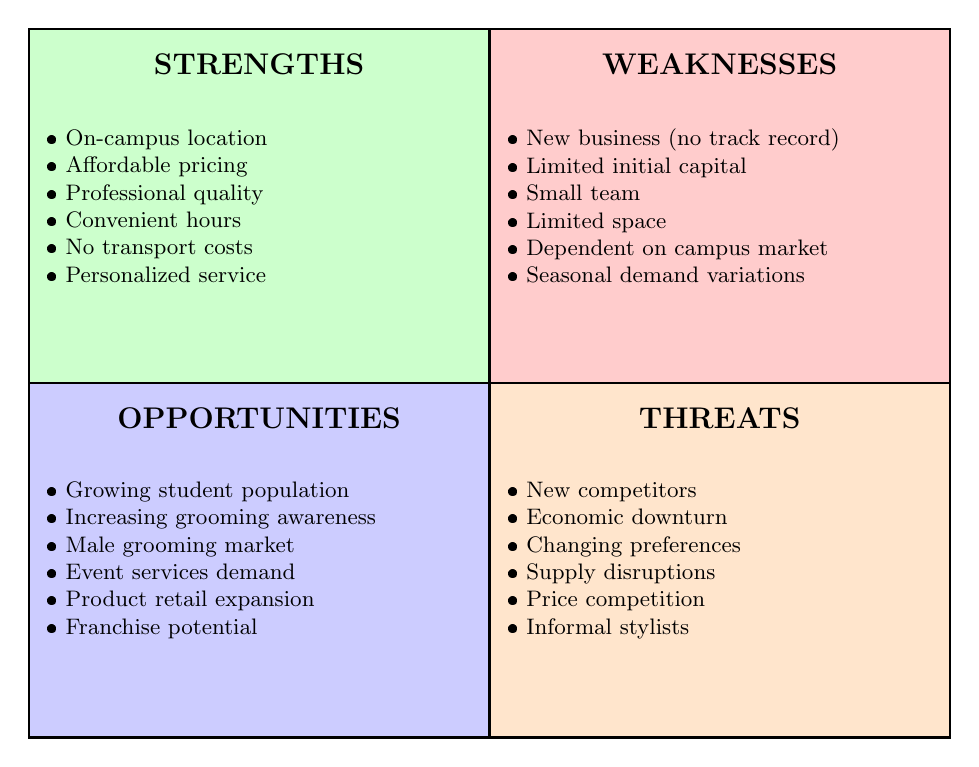
\begin{tikzpicture}[scale=0.9, transform shape]
    % Strengths (top left)
    \draw[fill=green!20, thick] (0,5) rectangle (6.5,10);
    \node at (3.25,9.5) [font=\bfseries\large] {STRENGTHS};
    \node at (3.25,7.5) [text width=6cm, align=left, font=\small] {
        • On-campus location\\
        • Affordable pricing\\
        • Professional quality\\
        • Convenient hours\\
        • No transport costs\\
        • Personalized service
    };
    
    % Weaknesses (top right)
    \draw[fill=red!20, thick] (6.5,5) rectangle (13,10);
    \node at (9.75,9.5) [font=\bfseries\large] {WEAKNESSES};
    \node at (9.75,7.5) [text width=6cm, align=left, font=\small] {
        • New business (no track record)\\
        • Limited initial capital\\
        • Small team\\
        • Limited space\\
        • Dependent on campus market\\
        • Seasonal demand variations
    };
    
    % Opportunities (bottom left)
    \draw[fill=blue!20, thick] (0,0) rectangle (6.5,5);
    \node at (3.25,4.5) [font=\bfseries\large] {OPPORTUNITIES};
    \node at (3.25,2.5) [text width=6cm, align=left, font=\small] {
        • Growing student population\\
        • Increasing grooming awareness\\
        • Male grooming market\\
        • Event services demand\\
        • Product retail expansion\\
        • Franchise potential
    };
    
    % Threats (bottom right)
    \draw[fill=orange!20, thick] (6.5,0) rectangle (13,5);
    \node at (9.75,4.5) [font=\bfseries\large] {THREATS};
    \node at (9.75,2.5) [text width=6cm, align=left, font=\small] {
        • New competitors\\
        • Economic downturn\\
        • Changing preferences\\
        • Supply disruptions\\
        • Price competition\\
        • Informal stylists
    };
    
\end{tikzpicture}
\caption{SWOT Analysis for Campus Glam Hub}
\end{figure}

\vspace{1.5em}

\begin{center}
\begin{tcolorbox}[mybox, title=\textbf{Strategic Implications of SWOT Analysis}, width=0.9\textwidth]
\textbf{Leverage Strengths:}
\begin{itemize}[leftmargin=1em, itemsep=2pt]
    \item Emphasize location advantage in all marketing
    \item Build reputation through consistent quality
    \item Use convenience as primary differentiator
\end{itemize}

\textbf{Address Weaknesses:}
\begin{itemize}[leftmargin=1em, itemsep=2pt]
    \item Build track record through excellent service
    \item Reinvest profits for expansion
    \item Cross-train staff for flexibility
    \item Diversify beyond campus market gradually
\end{itemize}

\textbf{Exploit Opportunities:}
\begin{itemize}[leftmargin=1em, itemsep=2pt]
    \item Develop male grooming service line
    \item Create event packages for graduations
    \item Expand product retail offerings
    \item Consider second location after Year 2
\end{itemize}

\textbf{Mitigate Threats:}
\begin{itemize}[leftmargin=1em, itemsep=2pt]
    \item Build strong customer loyalty
    \item Maintain cost efficiency
    \item Stay ahead of trends
    \item Secure reliable suppliers
\end{itemize}
\end{tcolorbox}
\end{center}

\vspace{1em}

\subsection{Business Model}

Campus Glam Hub operates on a service-based business model with supplementary retail sales:

\textbf{Revenue Streams:}
\begin{itemize}[leftmargin=2em]
    \item Service fees from beauty and grooming treatments (primary revenue)
    \item Retail sales of beauty products and accessories (secondary revenue)
    \item Special event packages and group bookings
    \item Membership or loyalty programs for regular customers
\end{itemize}

\textbf{Value Proposition:}
\begin{itemize}[leftmargin=2em]
    \item Convenience of on-campus location
    \item Affordable pricing for students
    \item Professional quality services
    \item Time-saving solution for busy students
    \item Personalized customer experience
\end{itemize}

\vspace{1em}

% Business Model Canvas Diagram
\begin{center}
\textbf{Business Model Canvas}
\vspace{0.5em}

\begin{tikzpicture}[scale=0.85, transform shape]
    % Define box style
    \tikzstyle{box}=[rectangle, draw=primarycolor, thick, fill=lightgray, text width=3.2cm, minimum height=2.5cm, align=center, font=\small]
    
    % Top row
    \node[box] at (0,0) (kp) {\textbf{Key Partners}\\Beauty product\\suppliers\\Equipment\\vendors\\University};
    \node[box] at (3.5,0) (ka) {\textbf{Key Activities}\\Service delivery\\Marketing\\Quality control\\Staff training};
    \node[box] at (7,0) (vp) {\textbf{Value Propositions}\\Convenient\\Affordable\\Professional\\Time-saving};
    \node[box] at (10.5,0) (cr) {\textbf{Customer Relations}\\Personal service\\Loyalty programs\\Social media\\Feedback};
    \node[box] at (14,0) (cs) {\textbf{Customer Segments}\\Students (80\%)\\Staff (15\%)\\Community (5\%)};
    
    % Bottom row
    \node[box] at (1.75,-3) (kr) {\textbf{Key Resources}\\Skilled staff\\Equipment\\Location\\Brand};
    \node[box] at (8.75,-3) (ch) {\textbf{Channels}\\Walk-in\\Appointments\\Social media\\Word-of-mouth};
    
    % Cost and Revenue
    \node[box, text width=6.5cm] at (1.75,-6) (cost) {\textbf{Cost Structure}\\Staff salaries, Rent, Products \& supplies,\\Utilities, Marketing, Equipment depreciation};
    \node[box, text width=6.5cm] at (8.75,-6) (revenue) {\textbf{Revenue Streams}\\Service fees (90\%), Product sales (10\%),\\Event packages, Loyalty memberships};
    
\end{tikzpicture}
\end{center}

\subsection{Products and Services}

\textbf{Core Services:}
\begin{itemize}[leftmargin=2em]
    \item \textbf{Hair Services:} Haircuts, styling, braiding, weaving, hair coloring, deep conditioning treatments, hair extensions
    \item \textbf{Makeup Services:} Event makeup, bridal makeup, photoshoot makeup, makeup consultations, makeup lessons
    \item \textbf{Skincare Services:} Facials, skin analysis, acne treatments, skin brightening treatments, moisturizing treatments
    \item \textbf{Nail Services:} Manicures, pedicures, nail art, gel nails, nail treatments
    \item \textbf{Other Grooming:} Eyebrow shaping, threading, eyelash extensions
\end{itemize}

\textbf{Retail Products:}
\begin{itemize}[leftmargin=2em]
    \item Hair care products (shampoos, conditioners, treatments)
    \item Skincare products (cleansers, moisturizers, sunscreens)
    \item Makeup products (foundations, lipsticks, eyeshadows)
    \item Beauty accessories (brushes, sponges, hair accessories)
\end{itemize}

